\documentclass{beamer}
\usetheme{Madrid}
\usepackage[turkish,shorthands=:!]{babel}
\usepackage{amsmath}
\usepackage{tikz}
\usetikzlibrary{babel,arrows.meta}

\title{Sunum Başlığı}
\subtitle{Alt başlık}
\author{Ad Soyad}
\institute{Kurum}
\date{\today}

\begin{document}

\begin{frame}
  \titlepage
\end{frame}

\begin{frame}{Türev: teğet doğrusunun eğimi}
  \begin{columns}
    \column{0.5\textwidth}
    \begin{itemize}
      \item $f'(a) = \lim\limits_{h\to 0}\dfrac{f(a+h)-f(a)}{h}$
      \item Teğet doğrusu: $y = f(a) + f'(a)(x-a)$
    \end{itemize}
    \column{0.5\textwidth}
    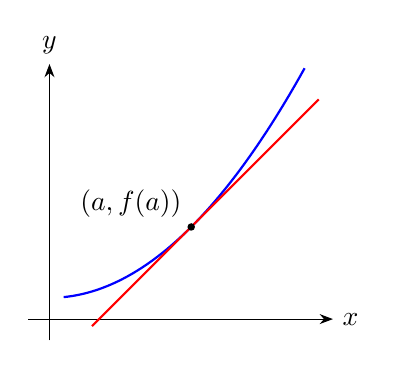
\begin{tikzpicture}[scale=0.9, >={Stealth}]
      \draw[->] (-0.3,0) -- (4,0) node[right] {$x$};
      \draw[->] (0,-0.3) -- (0,3.6) node[above] {$y$};
      \draw[thick, blue, domain=0.2:3.6, samples=50] plot (\x, {0.25*\x*\x + 0.3});
      \draw[thick, red, domain=0.6:3.8] plot (\x, {\x - 0.7});
      \fill (2,1.3) circle (1.5pt) node[above left] {$(a, f(a))$};
    \end{tikzpicture}
  \end{columns}
\end{frame}

\end{document}
